% Created 2020-07-15 mié 11:53
% Intended LaTeX compiler: pdflatex
\documentclass[presentation,aspectratio=169]{beamer}
\usepackage[utf8]{inputenc}
\usepackage[T1]{fontenc}
\usepackage{graphicx}
\usepackage{grffile}
\usepackage{longtable}
\usepackage{wrapfig}
\usepackage{rotating}
\usepackage[normalem]{ulem}
\usepackage{amsmath}
\usepackage{textcomp}
\usepackage{amssymb}
\usepackage{capt-of}
\usepackage{hyperref}
\usepackage{khpreamble}
\usepackage{amssymb}
\DeclareMathOperator{\shift}{q}
\DeclareMathOperator{\diff}{p}
\usetheme{default}
\author{Kjartan Halvorsen}
\date{\today}
\title{Control computarizado - Asignación de polos, controlador incremental}
\hypersetup{
 pdfauthor={Kjartan Halvorsen},
 pdftitle={Control computarizado - Asignación de polos, controlador incremental},
 pdfkeywords={},
 pdfsubject={},
 pdfcreator={Emacs 26.3 (Org mode 9.3.6)}, 
 pdflang={English}}
\begin{document}

\maketitle

\section{Intro}
\label{sec:org4b702ec}
\section{2-dof controller}
\label{sec:org6e0467a}
\begin{frame}[label={sec:orge365ea2}]{Controlador de dos grados de libertad}
\begin{center}
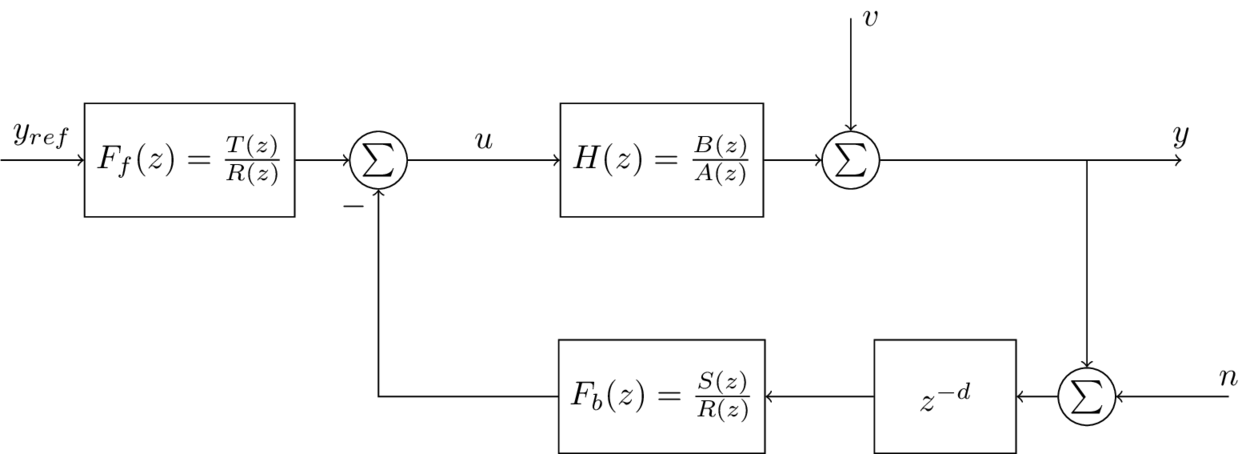
\includegraphics[width=0.7\linewidth]{../../figures/2dof-block-explicit}
\end{center}
\end{frame}
\section{Problem 5.3}
\label{sec:orgdfdc016}
\begin{frame}[label={sec:org7f71c1f}]{Åström \& Wittenmark problema 5.3}
Dado sistema
\[ H(z) = \frac{z+0.7}{z^2 -1.8z + 0.81} \]
Determina controlador de dos grados de libertad, dónde el polinomio caracteristica del sistema en lazo cerrado, desde la señal de referencia a la salida sea
\[ A_c(z) = z^2 - 1.5z + 0.7. \]
Pon los polos del observador en el origen (deadbeat observer). Considera tres casos
\begin{description}
\item[{(a)}] Control posicional \alert{con} cancelación del cero del proceso
\item[{(b)}] Control posicional \alert{sin} cancelación del cero del proceso
\item[{(c)}] Control \alert{incremental} sin cancelación del cero del proceso
\end{description}
\end{frame}

\begin{frame}[label={sec:org0d2bffa}]{¿Por qué cancelar el cero?}
Diagramas de Bode para los sistemas en lazo cerrado (seguimiento de referencia) con y sin cancelación del cero

\begin{center}
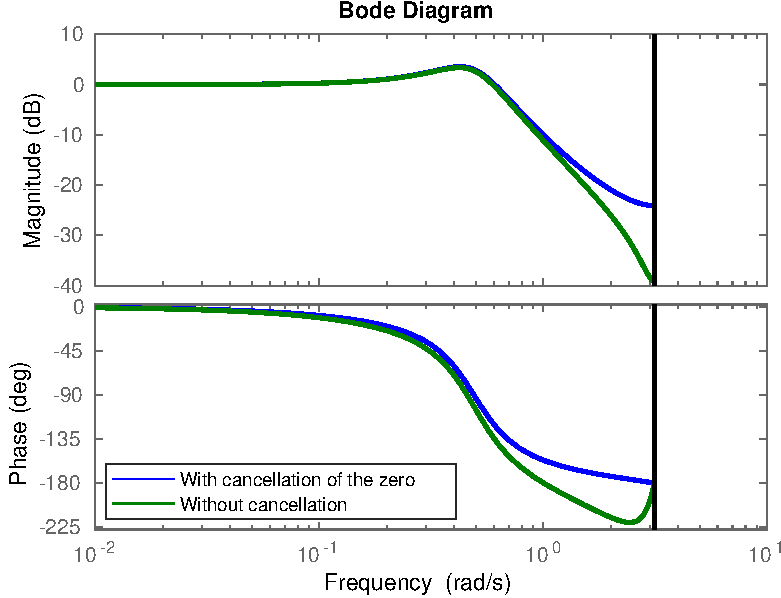
\includegraphics[width=0.6\linewidth]{../../figures/aw5_3_bode}
\end{center}
\end{frame}

\begin{frame}[label={sec:org55f820d}]{Ejercicio prelminario}
Cuál de las respuestas de sistema en lazo cerrado corresponde a (I) Control posicional \alert{con} cancelación del cero del proceso,  (II) Control posicional \alert{sin} cancelación del cero del, (III) Control \alert{incremental} sin cancelación del cero del proceso
\begin{center}
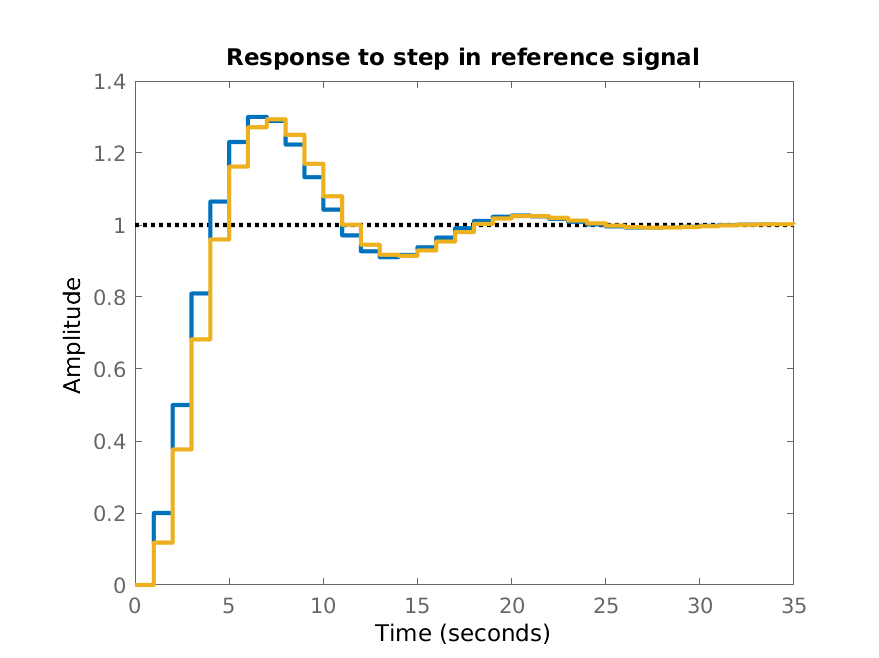
\includegraphics[width=0.45\linewidth]{../../figures/aw5_3_refstep}
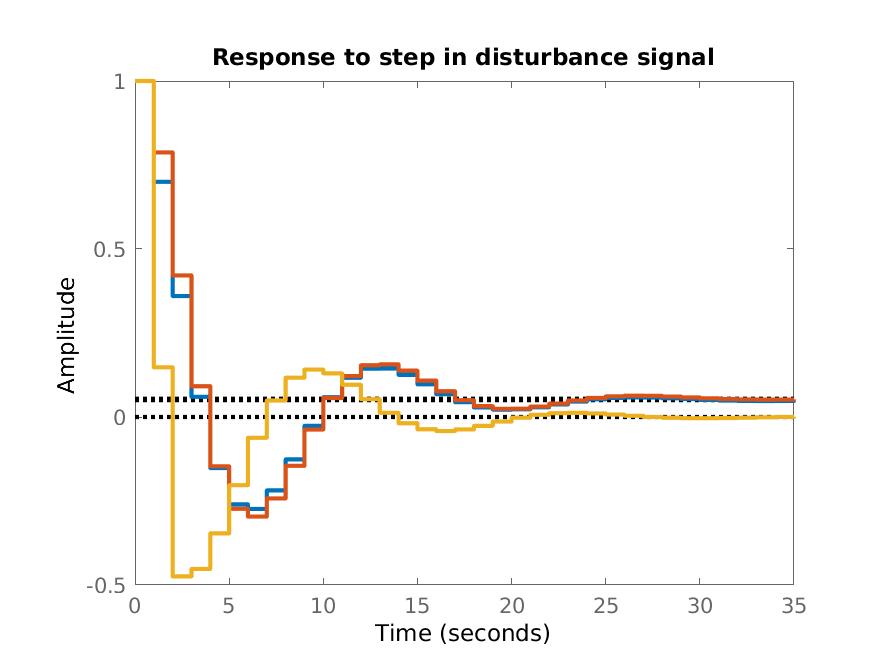
\includegraphics[width=0.45\linewidth]{../../figures/aw5_3_diststep}
\end{center}
\end{frame}

\begin{frame}[label={sec:org6642bf2}]{Soluciones}
\end{frame}
\begin{frame}[label={sec:orgbc8327f}]{Caso (a) Controlador posicional con cancelación del cero}
\begin{enumerate}
\item Eligimos el controlador \[F_b(z) = \frac{S(z)}{R(z)} = \frac{S(z)}{(z+1)\bar{R}(z)}\]
 para que haya cancelación del cero. Ecuación diofantina
\[A(z)(z+0.7)\bar{R}(z) + (z+0.7)S(z) = (z+0.7)A_c(z)A_o(z)\]
\[A(z)\bar{R}(z) + S(z) = A_c(z)A_o(z) \qquad (*)\]
Número de coeficientes desconocidos del controlador: \(2n_{\bar{R}} + 2\).
Número de ecuaciones de la ecuación diofantina: \(n_A + n_{\bar{R}}\).
\alert{\(\Rightarrow\qquad \(n_{\bar{R}} = n_{\deg A} - 2 = 2-2 = 0\)}
\[ F_{b}(z) = \frac{s_0z + s_1}{z+0.7}\]
\end{enumerate}
\end{frame}
\begin{frame}[label={sec:orgaff4374}]{Caso (a) Controlador posicional con cancelación del cero}
\begin{enumerate}
\setcounter{enumi}{1}
\item Factorización de \(A_{cl}(z) = A_c(z)A_o(z)\). Ecuación \((*)\) es de orden 2, igual  que \(A_c(z)\), entonces \alert{\(A_o(z) = 1\)}.
\end{enumerate}
\end{frame}
\begin{frame}[label={sec:org3eb4041}]{Caso (a) Controlador posicional con cancelación del cero}
\begin{enumerate}
\setcounter{enumi}{2}
\item Determina los polinomios \(R(z)\) y \(S(z)\). La ecuación diofantina
\[ (z^2 - 1.8z + 0.81) + s_0z + s_1 = z^2 - 1.5z + 0.7 \]
nos da el sistema de ecuaciones
\[ \begin{cases} z^1 :&  s_0 = -1.5+1.8= 0.3\\ z^0:& s_1 = 0.7-0.81=-0.11 \end{cases}\]
\alert{\[F_b(z) = \frac{0.3z - 0.11}{z + 0.7}\]}
\end{enumerate}
\end{frame}
\begin{frame}[label={sec:orga802c4a}]{Caso (a) Controlador posicional con cancelación del cero}
\begin{enumerate}
\setcounter{enumi}{3}
\item Determina  \[F_f(z) = \frac{T(z)}{R(z)} = \frac{t_0 A_o(z)}{B(z)}\]
Función de transferencia del seguimiento a la referencia:
\[ G_c(z) = \frac{ \frac{T}{R}\frac{B}{A}}{1 + \frac{B}{A} \frac{S}{R}} = 
                  = \frac{TB}{AR+BS} = \frac{t_0B}{BA_c} = \frac{t_0}{A_c}\]
Para obtener ganancia stática unitaria:
  \alert{\[ t_0 = A_c(1) = 0.2 \]}
\end{enumerate}
\end{frame}

\begin{frame}[label={sec:org708b3e9}]{Caso (b) Controlador posicional sin cancelación del cero}
\end{frame}

\begin{frame}[label={sec:orgb16fade}]{Caso (c) Controlador incremental sin cancelación del cero}
\end{frame}
\end{document}